\documentclass[tikz,border=0.0in]{standalone}
\usepackage{tikz}   
\usepackage{tikzscale}
\usepackage{amsmath}
\usetikzlibrary{arrows.meta, positioning}

\begin{document}

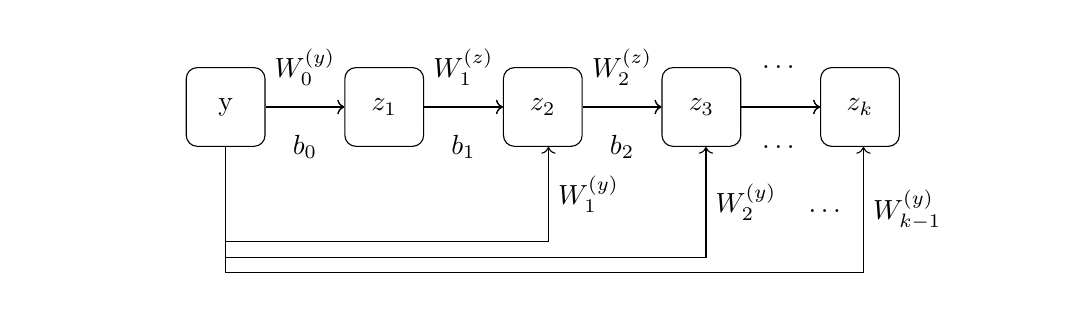
\begin{tikzpicture}[
    node distance=1cm and 1cm,
    every node/.style={rounded corners, minimum width=1cm, minimum height=1cm, align=center}
]

    % Nodes
    %\node[draw=none,fill=none] (topmargin) at (0,1.1) {};  % top spacer

    \node[draw=none,fill=none] (start) {};
    \node[draw, right=of start] (y) {y};
    \node[draw, right=of y] (z1) {$z_1$};
    \node[draw, right=of z1] (z2) {$z_2$};
    \node[draw, right=of z2] (z3) {$z_3$};
    \node[draw, right=of z3] (zk) {$z_k$};
    \node[right=of zk,draw=none,fill=none] (end) {};
    \node[draw=none,fill=none,below=1cm of y] (bottommargin) {}; % bottom spacerS
    

    % Forward Weights
    \draw[->] (y) -- node[above] {$W_0^{(y)}$} (z1);
    \draw[->] (z1) -- node[above] {$W_1^{(z)}$} (z2);
    \draw[->] (z2) -- node[above] {$W_2^{(z)}$} (z3);
    \draw[->] (z3) -- node[above] {$\dots$} (zk);

    % Biases
    \draw[->] (y) -- node[below] {$b_0$} (z1);
    \draw[->] (z1) -- node[below] {$b_1$} (z2);
    \draw[->] (z2) -- node[below] {$b_2$} (z3);
    \draw[->] (z3) -- node[below] {$\dots$} (zk);

    % Right-Angled Recurrent Connections (Down -> Right -> Up)
    \draw[->] (y.south) -- ++(0,-1.2) -- ++(4.1,0) -- ++(0,1.2) node[midway, right] {$W_1^{(y)}$} (z2);
    \draw[->] (y.south) -- ++(0,-1.4) -- ++(6.1,0) -- ++(0,1.4) node[midway, right] {$W_2^{(y)}\quad \dots$} (z3);
    \draw[->] (y.south) -- ++(0,-1.6) -- ++(8.1,0) -- ++(0,1.6) node[midway, right] {$W_{k-1}^{(y)}$} (zk);
\end{tikzpicture}

\end{document}